 %===================================== CHAP 5 =================================

\chapter{Architecture and implementation, Not finished}
\label{ch:architecture_and_implementation}

\section{User interface}
\label{sec:architecture_and_implementation-user_interface}

One of the initial requirements from the customer, was to have a graphical user interface. It was supposed to display relevant data and allow the administrator to moderate topics and subscriptions. After an initial consideration, the Spring Framework\footnote{\url{http://projects.spring.io/spring-boot/}} was chosen to be the most suitable framework ( \ref{subsec:prestudies-tools-spring_mvc}) for building the administration panel. The user interface was implemented using the MVC-pattern. 

\subsection{Design}
\label{subsec:architecture_and_implementation-user_interface-design}

\begin{center}
  \begin{figure}[ht!]
    \makebox[\textwidth]{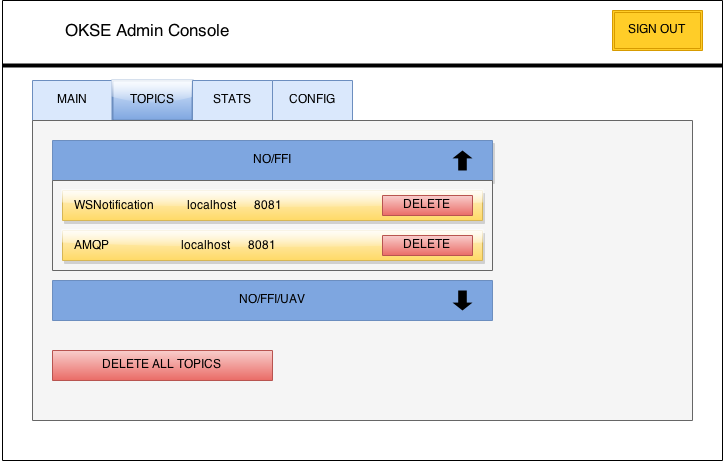
\includegraphics[scale=0.5]{fig/initial_prototype.png}}
    \caption{Initial website wireframe}
    \label{fig:initial_prototype}
  \end{figure}
\end{center}

A considerable amount of time were spent researching the Apollo broker during the research phase, which provided information about what such an interface should provide. Originally the customer had not stated any specific requirements for the administration panel. Therefore, an initial website wireframe was created, and shown to the customer. The wireframe was heavily influenced by Apollo. This wireframe (fig \ref{fig:initial_prototype}), along with the creation of use cases, set the terms for creating a prototype.

The group agreed upon creating a functional prototype for the customer. This prototype was made available, so that the customer could provide feedback. During most customer meetings, the current version of the administration panel was discussed. The customer gave feedback on how new elements in the panel met the customers expectations. This approach gave the group one big advantage; rapid response from the customer which made it easy to improve the interface and add additional features. Throughout the lifetime of the development phase, the administration panel were continuously released and deployed on the test server.

The final interface contained six panes; "Main", "Topics", "Subscribers", "Statistics", "Logs" and "Configuration". The "Main"-pane contains information about the message broker. It is meant to give a general overview of the current operating environment, as well as the system status, such as memory usage. The "Statistics"-pane contain useful statistics about requests, messages etc. on the different protocols. The "Logs"-pane contains runtime logs for debugging purposes. The "Topics"-pane shows all registered topics in the message broker. On this pane, information about the current topics, as well as the possibility to remove them. The "Subscribers"-pane has exactly the same functionality as the "Topics"-pane, but it's for subscribers. Finally, in the "Configuration"-pane, the user can change the brokers settings and map topics together. Also, a possibility to add relays between multiple OKSE brokers is located here. 

\subsection{Implementation}
\label{subsec:architecture_and_implementation-implementation}

The front-end was designed in a modularized way, where one controller class was responsible for one pane. The advantage of this approach was having the administration panel designed as a single page web application. The page uses AJAX-requests to reach a representational state transfer (hereby denoted as REST) API. By using the Spring Framework, the system exposes API-endpoints which can be used to access and/or modify data. This is used as the main data source for the front-end and is a critical part of the single page design. Translated to the MVC-pattern, the Spring Framework works as a controller through REST-controllers, and the different panes works as views. Each AJAX-request to the API-endpoints will reach the controllers and modify the models and/or message broker. Structuring the system this way gave some advantages: 

\begin{itemize}
    \item No need to refresh the entire administration panel.
    \item One controller class served one pane; easy to debug.
    \item Loose coupling, no dependencies between panes.
    \item Easy to extend the application further.
\end{itemize}

\subsubsection{Architecture}

\begin{center}
  \begin{figure}[ht!]
    \makebox[\textwidth]{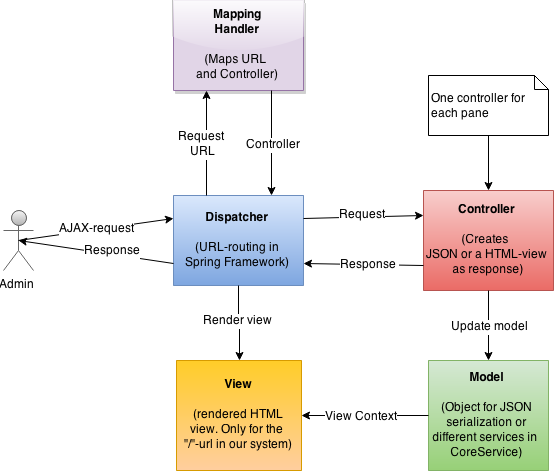
\includegraphics[scale=0.5]{fig/spring.png}}
    \caption{REST-API architecture}
    \label{fig:spring}
  \end{figure}
\end{center}

Figure \ref{fig:spring} shows an overview of how a request is handled by the server. The main workflow is as follows:

\clearpage

\begin{itemize}
    \item\textbf{Dispatcher} -  This is the class that is exposed to the user. It forwards request URL's to the mapping handler to reach the correct controller. It then calls the controller responsible for the request. Finally it returns the response to the user. 
    \item\textbf{Mapping handler} - This class maps the request URL to the controller responsible for the request, and returns it to the dispatcher. 
    \item\textbf{Controller} - This is the class responsible for executing tasks and getting information from the message broker. It returns a JSON\footnote{\url{http://www.json.org/}} response string to the dispatcher.  
\end{itemize}

\section{Broker architecture}
\label{sec:architecture_and_implementation-broker_architecture}

This section discusses the high-level aspects of the broker architecture. Some parts of the system are explained in greater detail to provide clear purpose or intent.

\subsection{Goals and strategy}
\label{subsec:architecture_and_implementation-broker_architecture-goals_and_strategy}

Building on the results and findings in the research phase, the team created a set of goals for the design of the system architecture. Several aspects of the Apollo broker were really well thought out, and were on the priority list from the start. These included, but were not limited to: Complete protocol agnostic interface. A priority message queue supported by a multi-threaded execution service. Loose coupling of modules, as well as high extendability and low maintenance effort.

Expanding on these traits, the group wanted a system architecture where each component was a standalone service. A service would expose a public interface from which other components could request data access or services from. Another goal of the design was to have a core service responsible for registering other services, starting them, stopping them, and registering protocols. This would allow the system to be extended by simply registering the new component, without further modifications.

The customer had requested a graphical user interface, and building on the experience and knowledge in the group, a web based interface was deemed most appropriate. The group wanted to have an administration interface built using the dynamic properties of the outlined system. Registering a new protocol should not require the administration interface component to be modified. Registering a new core service that a potential developer wanted to expose in the admin interface, should only require adding a new model, API controller and template fragment.

Based on these thoughts and ideas, a list of goals were created:

\begin{itemize}
\item The system shouldn't need to know about the details of registered protocols in order to perform as intended. In essence, it should be completely protocol agnostic.
\item Extending the system with new functionality should be as easy as possible.
\item Extending the system with new protocols should be as easy as possible.
\item Extending the system should require as little alteration to existing code as possible.
\item Core functionality should be adhering to the principle of "Separation of concerns".
\item Core services should be standalone entities that other components can utilize.
\item The system should have a core service responsible for the entire life cycle of other registered components.
\end{itemize}

\begin{center}
  \begin{figure}[ht!]
    \makebox[\textwidth]{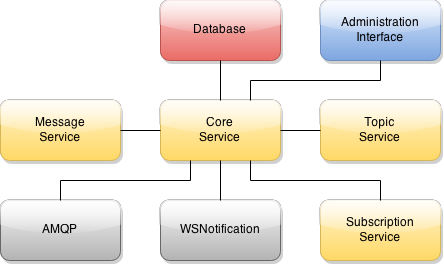
\includegraphics[scale=0.6]{fig/abstract_architecture.png}}
    \caption{High-level system architecture}
    \label{fig:abstract_architecture}
  \end{figure}
\end{center}

With these goals settled, it was apparent that the design outline had properties of a Service Oriented Architecture\footnote{\url{http://en.wikipedia.org/wiki/Service-oriented_architecture}} (hereby denoted as SOA), as well as the Module Pattern\footnote{\url{http://en.wikipedia.org/wiki/Module_pattern}}. This prompted the actual implementation of the system to adhere to these principles and patterns as much as possible, for consistency and future familiarity.

Putting all this together, a high-level system architecture was created (fig \ref{fig:abstract_architecture}). It illustrates the main entities that were to become the brokering system. Lines between entities illustrate their connection to the core service, which is responsible for all other entity life cycles. Yellow entities are core services in the brokering system, while gray are protocol components.

\subsection{Component dependency}
\label{subsec:architecture_and_implementation-broker_architecture-component_dependency}

The next step was to identify possible critical dependencies and usage dependencies required for a component to provide its complete set of features. This meant that a wide range of scenarios and situations, data flows and potential class structures had to be evaluated. By using the principles of SOA and Module Pattern, the amount of critical dependencies were reduced to a minimum.

Usage dependency could however, not be reduced to a level lower than what was needed for the system to operate as intended. It was also planned to use event callbacks to handle situations that would have caused extra inter-service dependencies. This would allow services to run regardless of their real-world dependency on other services during certain tasks. An example of this is a situation where a topic is deleted in the administration interface, and subscribers have to be purged from the subscription service. The solution was to have the subscription service listen for topic-related events and update its subscriber set accordingly.

\begin{center}
  \begin{figure}[ht!]
    \makebox[\textwidth]{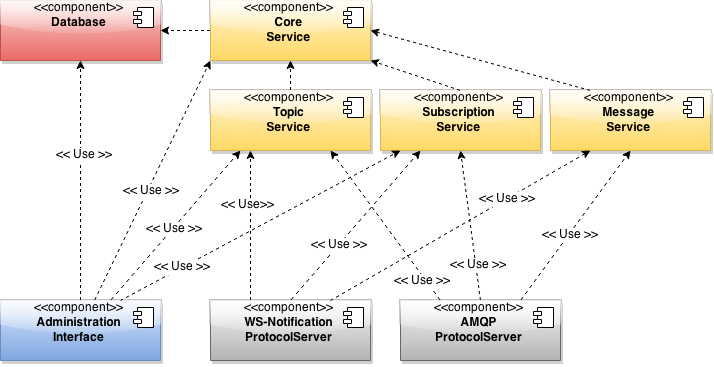
\includegraphics[scale=0.5]{fig/architecture_dependency.png}}
    \caption{Component Dependencies}
    \label{fig:architecture_dependency}
  \end{figure}
\end{center}

After much thought was put into these challenges, a component dependency diagram (fig \ref{fig:architecture_dependency}) was created to illustrate how the administration interface, services and protocols should depend on each other. As with the high-level architecture, core services are denoted with yellow and protocols with gray.

Dependencies between components that are annotated with $<< Use >>$ represents situations where a component depends on the other to offer its full set of features. In practice, a complete implementation of the brokering system would rely on all these dependencies to meet the specified requirements. But they should not be required for a component to perform its own internal responsibilities. Hence, a single instance of the WSN protocol should be able to run without connectivity to the rest of the system, and fully function in its local environment. This would however, mean that the rest of the system would be unaware of the subscribers, topics and messages handled by the local instance.

\clearpage

\subsection{Data flow}
\label{subsec:architecture_and_implementation-broker_architecture-data_flow}

\begin{center}
  \begin{figure}[ht!]
    \makebox[\textwidth]{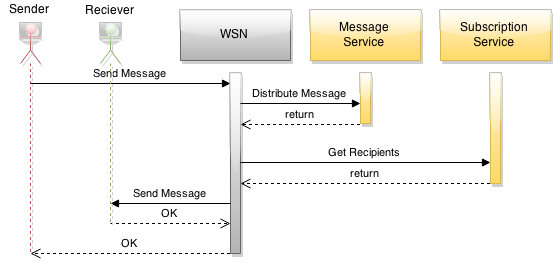
\includegraphics[scale=0.6]{fig/architecture_data_flow_simple.png}}
    \caption{Simplified sequence diagram of possible data flow when sending a notification message using WS-Nu as the protocol library.}
    \label{fig:architecture_data_flow_simple}
  \end{figure}
\end{center}

During the analysis of component dependencies, several potential data flows were analysed. They were used as references when evaluating what components would have critical dependencies and usage dependencies. This proved helpful, as the complexity and scope of what the group had to take into consideration begun to dawn at that point. An example of one of these data flows is a possible notification message being sent. A simplified version of the data flow is illustrated in figure \ref{fig:architecture_data_flow_simple}.

The figure illustrates which system calls are needed for a sender to send a message, process it, and deliver it. In practice, there might be several receivers and many additional calls, but this has been abstracted away for simplicity.

These simplified sequences were expanded later on, to provide a more realistic data flow in greater detail. During development, the detailed sequences were used as support when implementing proper start up sequences of the different components. Additionally, they were helpful in identifying possible computational bottlenecks, and provide insight into different ways of structuring the code.

\clearpage

\begin{center}
  \begin{figure}[ht!]
    \makebox[\textwidth]{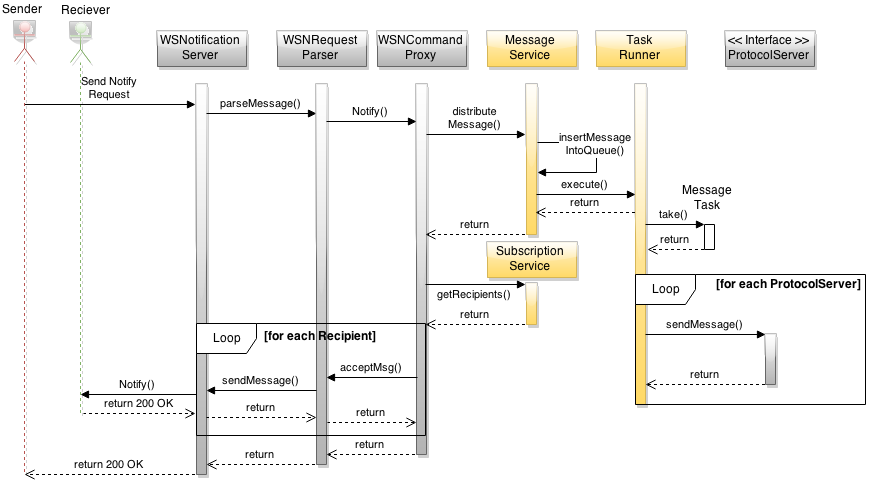
\includegraphics[scale=0.45]{fig/architecture_data_flow.png}}
    \caption{Detailed sequence diagram of possible data flow when sending a notification message using WS-Nu as the protocol library.}
    \label{fig:architecture_data_flow}
  \end{figure}
\end{center}
Figure \ref{fig:architecture_data_flow} illustrates an expanded version of what the potential data flow might look like for a send notification message request using WSN. The expanded data flows show occurrences of loops, as well as some of the ideas for inner workings of the components. In this example, the send message call performed in the task runner would invoke a large branch of actions itself. To reduce complexity, the analysis of potential data flows were divided into different segments of the proposed system architecture.


\section{Implementation}
\label{sec:architecture_and_implementation-implementation}

\subsection{Core}
\label{subsec:architecture_and_implementation-implementation-core}

\subsection{Topic and Queue difference}
\label{subsec:architecture_and_implementation-topic_and_queue_differecnce}
While the publish/subscriber pattern and WSN uses the concept topic to describe where a message is suppose to be routed, AMQP uses the concept of queues. As there is quite a big fundamental difference between them, a description of each can be found below. Both description is of the basic idea for the concepts.

\subsubsection{Topic}
When a system is implemented with the behaviour of topics, a incoming message will be distributed to every subscriber on the given topic. This means that if the topic "example" has three subscribers, and a message is sent to this topic, the message will be sent to all the subscribers.

\subsubsection{Queue}
When a system is implemented with the behaviour of a queue, a incoming message will be distributed to \textit{one} of the subscribers on the given queue. This means that if the queue has three subscribers, and message is sent to this queue, the message will be sent to \textit{one} of the subscriber. The way the subscriber is chosen can be implemented in a number of ways, two examples is at random, and using a round-robin algorithm\footnote{\url{http://en.wikipedia.org/wiki/Round-robin}}. A typical usage for queue based messaging  protocols is load balancing, which works out of the box when using queues.

\subsection{WSN}
\label{subsec:architecture_and_implementation-implementation-wsn}

Here be information about how WSN was implemented, as well as how it works

\subsection{AMQP}
\label{subsec:architecture_and_implementation-implementation-amqp}
The implementation of AMQP consists of mainly two parts. The first part is the handling of AMQP decoding and encoding of messages and the handling of the AMQP data in the network requests and responses. The second part is the handling of broker behaviour and the integration with the rest of the system. 

As every protocol server is implemented to run on a single thread, there was a need to handle the incoming and outgoing requests/messages in a clever way. After some consideration, the AMQP protocol server was implemented using the reactor event loop pattern\footnote{\url{http://en.wikipedia.org/wiki/Reactor_pattern}}\footnote{\url{http://en.wikipedia.org/wiki/Event_loop}}. 
The AMQP network socket was implemented using the Java non-blocking I/O library. The benefits of using a non-blocking socket is that instead of creating one socket per client, it will instead open multiple channels on one socket by using multiplexing. This is ideal for the single thread approach, as it runs in non-blocking mode, and will run in the main thread without stopping the entire program. The reactor pattern works well in combination with a multiplexed socket, as one of the key features of the pattern is the handling of incoming data from multiple sources. After the input is received and has been demultiplexed, Qpid will convert the incoming data to an event, which is then added to the event queue.

Simultaneously as the event queue gets new events, the event loop is continuously dispatching the events to the correct methods on different handlers. A handler is a class that extends the \verb!BaseHandler! class from Qpid. The handler can override event methods invoked by the event queue. The AMQP implementation has the following handlers; \verb!AMQPServer!, \verb!Driver!, \verb!Handshaker! and \verb!SubscriptionHandler!, with their own specific task.

\begin{center}
  \begin{figure}[ht!]
    \makebox[\textwidth]{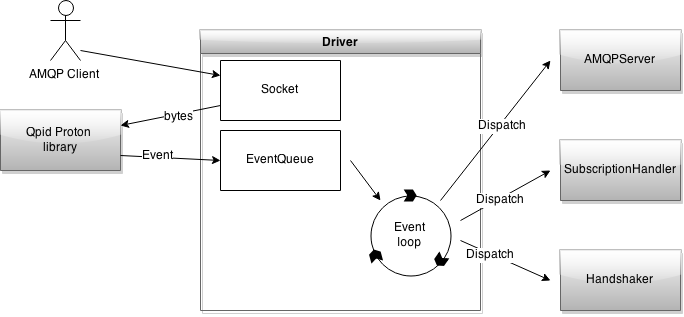
\includegraphics[width=\textwidth]{fig/amqp_recv.png}}
    \caption{AMQP Receive implementation overview}
    \label{fig:abstract_architecture}
  \end{figure}
\end{center}

\subsubsection{AMQPServer}
The AMQPServer handler is responsible for the incoming and outgoing messages. It handles the messages that come from AMQP producers and the internal messages from other protocols. It has an internal message queue where messages is stored until the corresponding event is triggered. It handles conversion of messages from AMQP format to the OKSE internal representation, and dispatching to the message service. It is implemented with optimizations to get AMQP messages out fast, and to prevent loops. When an AMQP message is received, it will automatically dispatch the AMQP message back to AMQP subscribers, and the OKSE message to the WSN subscribers.

\subsubsection{Driver}
The event loop and the socket logic is implemented in the Driver class. This class is responsible for accepting incoming connections, and handle the incoming requests. After a connection is opened with a client, every request received is passed to Qpid, which decodes the instruction and adds it back to the Driver in the form of an event. The event is added straight to a collector, which is used as the event queue. The event loop that is running continuously, will dispatch events as long as there are any in the queue. If there are no events, it will enter a wait state.

\subsubsection{SubscriptionHandler}
In the SubscriptionHandler class, the handling of subscribers and their routes/topics is handled. Additionally, it handles the basic information about a sender/producer and the integration with the systems centralized subscriber system. The functionality in this handler is based on addition and removal of subscribers. When a subscribe request occurs, the handler will add the user to the internal subscriber map, the system wide subscriber database and update the administration interface accordingly. When a subscriber disconnects, it removes the disconnected subscriber in the same manner.

\subsubsection{Handshaker}
The Handshaker handles all of the open and close events of a connection. It makes sure that the initiation of the connection, session and link is done properly. It also ensures that it is closed properly when the link is broken or disconnected.

\begin{center}
  \begin{figure}[ht!]
    \makebox[\textwidth]{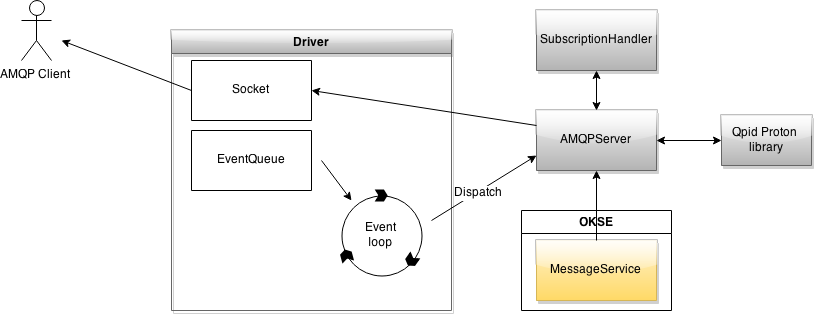
\includegraphics[width=\textwidth]{fig/amqp_send.png}}
    \caption{AMQP Send implementation overview}
    \label{fig:abstract_architecture}
  \end{figure}
\end{center}

\subsubsection{Queue vs Topic behavior}
WSN and AMQP use different behaviours for handling topics/queues. As WSN is a pure publish/subscribe protocol, it is only concerned with topics. A description of the difference between topics and queues can be found in \ref{subsec:architecture_and_implementation-topic_and_queue_differecnce}.

In the initial implementation, the system only complied with the given standards for each protocol. To cope with the differences, the group implemented logic to handle the conversion between the two behaviours. In addition, the group consulted the customer with the idea of implementing a non-standard topic implementation of AMQP. This meant that they could use AMQP with the same behaviour as WSN, and that all AMQP subscribers on one topic/queue would get the message. The customer liked the idea of this feature as they thought this would fit nicely with their use pattern.

A configuration switch was implemented to select which mode to use. The switch is available through the configuration file and the web administration interface. The logic for this feature is implemented in AMQPServer, which as previously stated is responsible for the outgoing message logic.



\clearpage
